%%%%%%%%%%%%%%%%%%%%%%%%%%%%%%%%%%%%%%%%%%%%%%%%%%%%%%%%%%%%%%%%%%%%%%%%%%%%%%%%
% metodologia.tex
%
% Capítulo de metodologia da monografia.
%%%%%%%%%%%%%%%%%%%%%%%%%%%%%%%%%%%%%%%%%%%%%%%%%%%%%%%%%%%%%%%%%%%%%%%%%%%%%%%%

\chapter{Metodologia}
\label{sec:metod}

Este capítulo descreve a metodologia adotada no desenvolvimento do
trabalho, explicando a natureza da pesquisa, a abordagem metodológica, o
contexto do estudo, as etapas executadas e a estratégia de análise dos
resultados. O trabalho insere-se na área de Sistemas de Informação e tem
como foco a proposição e implementação de uma solução de automação do
fluxo pedagógico no sistema Educa EMES, utilizado pela Escola da
Magistratura do Espírito Santo (EMES).

\section{Natureza da pesquisa}
\label{sec:metod:natureza}

O trabalho caracteriza-se como uma pesquisa aplicada, voltada à solução
de um problema concreto relacionado à gestão educacional e à automação
de processos institucionais \cite{CreswellCreswell2023}. No contexto deste
estudo, essa caracterização decorre do fato de a investigação estar orientada à
identificação de lacunas no sistema existente, à modelagem de melhorias
e à implementação de mecanismos capazes de ampliar a automação do fluxo
pedagógico em ambiente institucional real.

\section{Abordagem metodológica}
\label{sec:metod:abordagem}

A abordagem metodológica adotada é predominantemente qualitativa, pois o interesse do
trabalho está na compreensão dos impactos da solução proposta sobre os
processos pedagógicos da EMES, observando aspectos como integração entre
etapas, padronização de rotinas, redução de intervenções manuais e
eficiência operacional. A ênfase analítica recai sobre a interpretação
do comportamento do fluxo pedagógico e sobre os efeitos das
intervenções propostas no processo organizacional
\cite{CreswellCreswell2023}.

\section{Contexto e objeto do estudo}
\label{sec:metod:contexto}

A Escola da Magistratura do Espírito Santo (EMES) é uma instituição
vinculada ao Poder Judiciário, responsável pela formação e capacitação
de magistrados, servidores e demais públicos externos ou vinculados ao
judiciário. O sistema Educa EMES, desenvolvido em contexto real de
aplicação institucional, constitui uma solução integrada de gestão
educacional que abrange módulos de gestão acadêmica, administrativa,
contratação, orçamento, documentação, mensageria e comunicação. O
sistema já contempla funcionalidades básicas do fluxo pedagógico, como
inscrição em cursos, controle de frequência, aprovação e emissão de
certificados, mas apresenta limitações quanto à automação completa do
ciclo acadêmico.

O objeto do estudo delimita-se à automação do fluxo pedagógico dentro
do sistema Educa EMES, tratando-o simultaneamente como ambiente base da
solução proposta e como estudo de caso aplicado à gestão educacional em
instituição pública \cite{Yin2018}. O foco concentra-se nos processos de inscrição,
frequência, aprovação, certificação e geração de relatórios, com ênfase
na redução de intervenções manuais e na padronização de procedimentos,
aspectos diretamente associados à automação e à orquestração de
processos.

\section{Etapas de análise do fluxo pedagógico}
\label{sec:metod:etapas}

As etapas do desenvolvimento do trabalho foram executadas de forma
sequencial, alinhadas aos objetivos específicos definidos no capítulo
anterior. A seguir, são descritas as etapas de análise do fluxo
pedagógico.

\subsection{Análise do fluxo pedagógico atual da EMES no contexto de utilização do sistema Educa EMES}
\label{sec:metod:etapas:analise_fluxo}

Esta etapa consistiu na análise detalhada do fluxo pedagógico atual da
EMES, considerando o contexto de utilização do sistema Educa EMES. O
fluxo pedagógico foi mapeado a partir da observação das rotinas
institucionais e da interação com o sistema existente, identificando as
etapas principais do ciclo de vida de um curso ou evento educacional.

O processo inicia-se com o planejamento do curso pelo coordenador
pedagógico, que insere informações básicas em uma planilha de
cronograma, incluindo data, ministrante, local e título. Em seguida, o
curso é cadastrado no sistema Educa EMES com dados mais completos, como
horários exatos, carga horária, divisão de atividades, critérios de
certificação, tolerâncias para frequência, informações sobre
instrutores, local de realização, modalidade, senhas ou links de
acesso.

Após o cadastro, ocorre a abertura e encerramento de inscrições,
análise dos pré-inscritos e confirmação das inscrições com base em
critérios como setor ou vínculo com o Poder Judiciário. A confirmação
automática gera registros de frequência e dispara e-mails de
confirmação aos alunos. Conforme o curso se aproxima, o sistema envia
lembretes automáticos por e-mail (3 e 1 dia antes) às 6h da manhã.

Durante a execução do curso, os alunos registram frequência, e ao
término, um servidor da EMES utiliza uma ferramenta do sistema para
aprovar ou reprovar alunos conforme critérios de aprovação e presença.
Posteriormente, outro servidor gera certificados para alunos e
instrutores, considerando modalidades como certificado por atividade,
para o evento completo ou com carga horária somada das atividades
participadas.

Após a geração, os alunos recebem e-mail com link para formulário de
avaliação, e ao preenchê-lo, o certificado é disponibilizado na área do
aluno. O ciclo encerra-se com a geração de relatórios mensais para
acompanhamento de metas, incluindo cursos realizados, número de
inscritos, taxa de evasão e magistrados capacitados, mediante
exportação manual de dados do sistema.

Esta análise permitiu compreender a estrutura atual do fluxo
pedagógico, identificando pontos de integração com o sistema Educa EMES
e estabelecendo base para as etapas subsequentes.

\subsection{Identificação dos pontos de intervenção manual e as limitações de automação existentes nas etapas do processo acadêmico}
\label{sec:metod:etapas:intervencao_manual}

Esta etapa envolveu a identificação sistemática dos pontos de
intervenção manual e das limitações de automação existentes no fluxo
pedagógico, com base na análise realizada na etapa anterior. Foram
observadas as rotinas que ainda dependem de ação direta dos servidores,
mesmo com o sistema Educa EMES em operação, focando nas limitações que
não podem ser automatizadas ou seriam muito trabalhosas para pouco
ganho.

O principal ponto de limitação identificado refere-se ao cadastro
inicial do curso no sistema, durante a transição da planilha de
cronograma para o Educa EMES. Essa tarefa apresenta complexidade para
automação, pois envolve decisões contextuais e contato com terceiros
para obtenção de informações adicionais, tornando a automatização
completa pouco viável. No entanto, foi identificado que a validação da
integridade do cadastro pode ser monitorada pelo sistema, verificando
se os campos mínimos necessários estão preenchidos para evitar
pendências durante a execução do curso.

\subsection{Identificação dos gargalos e as oportunidades de melhoria no fluxo pedagógico da EMES}
\label{sec:metod:etapas:gargalos}

Esta etapa concentrou-se na identificação dos gargalos existentes no
fluxo pedagógico e na exploração de oportunidades de melhoria,
fundamentada nas análises das etapas anteriores. Os gargalos foram
classificados em categorias principais, com ênfase em problemas
recorrentes que impactam a eficiência operacional e podem ser
endereçados através de automação.

O primeiro gargalo refere-se à integridade do cadastro e conflitos de
informações, onde é comum o esquecimento de campos essenciais durante o
cadastro, como senhas para salas remotas ou datas de inscrição. Isso
resulta em cadastros inconsistentes com a carga horária ou
agendamentos conflitantes, gerando confusão durante a execução do curso
e necessidade de correções posteriores.

O segundo gargalo envolve a gestão do processo de inscrição, onde
servidores frequentemente esquecem de abrir ou fechar inscrições, ou
cadastram datas incorretas, comprometendo o controle temporal das
vagas.

O terceiro gargalo diz respeito à confirmação manual de inscrições em
cursos com públicos-alvo específicos, que requerem análise individual
de perfis, consumindo tempo e gerando inconsistências.

O quarto gargalo relaciona-se à aprovação de alunos e inconsistência de
critérios, principalmente em eventos com múltiplas atividades, onde
erros de aprovação parcial ou desentendimentos entre responsáveis pelo
cadastro e aprovação geram retrabalho.

O quinto gargalo concerne à geração de certificados inconsistentes com
o cadastro, onde divergências entre a modalidade projetada e a
executada resultam em retrabalho e insatisfação.

Finalmente, o sexto gargalo refere-se à geração de relatórios, onde
demandas pontuais sobrecarregam a equipe, exigindo interrupção de outras
atividades para extração manual de dados.

Esses gargalos representam oportunidades de melhoria através da
automação, como validações automáticas de cadastro, alertas para gestão
de inscrições, confirmações inteligentes, padronização de critérios de
aprovação, geração automática de certificados e relatórios dinâmicos,
contribuindo para maior eficiência e redução de erros no fluxo
pedagógico \cite{Weske2024}.

\subsection{Representação BPMN do fluxo pedagógico atual}
\label{sec:metod:etapas:bpmn-as-is}

Como forma de consolidar visualmente a análise do fluxo pedagógico atual,
foi elaborado um diagrama BPMN representando o processo \textit{AS-IS},
ou seja, a forma como o fluxo ocorre no contexto atual de utilização do
sistema Educa EMES. O diagrama organiza o processo em raias
correspondentes à coordenação, à equipe pedagógica, ao sistema Educa
EMES, ao instrutor e ao aluno, permitindo identificar com maior clareza
as responsabilidades distribuídas ao longo do ciclo do curso. Nesse
contexto, o instrutor é representado como participante do processo
pedagógico, mas não como ator funcional da automação proposta.

\begin{figure}[H]
\centering
\caption{Representação BPMN do fluxo pedagógico atual (\textit{AS-IS})}
\label{fig:bpmn-as-is}
  \fbox{
     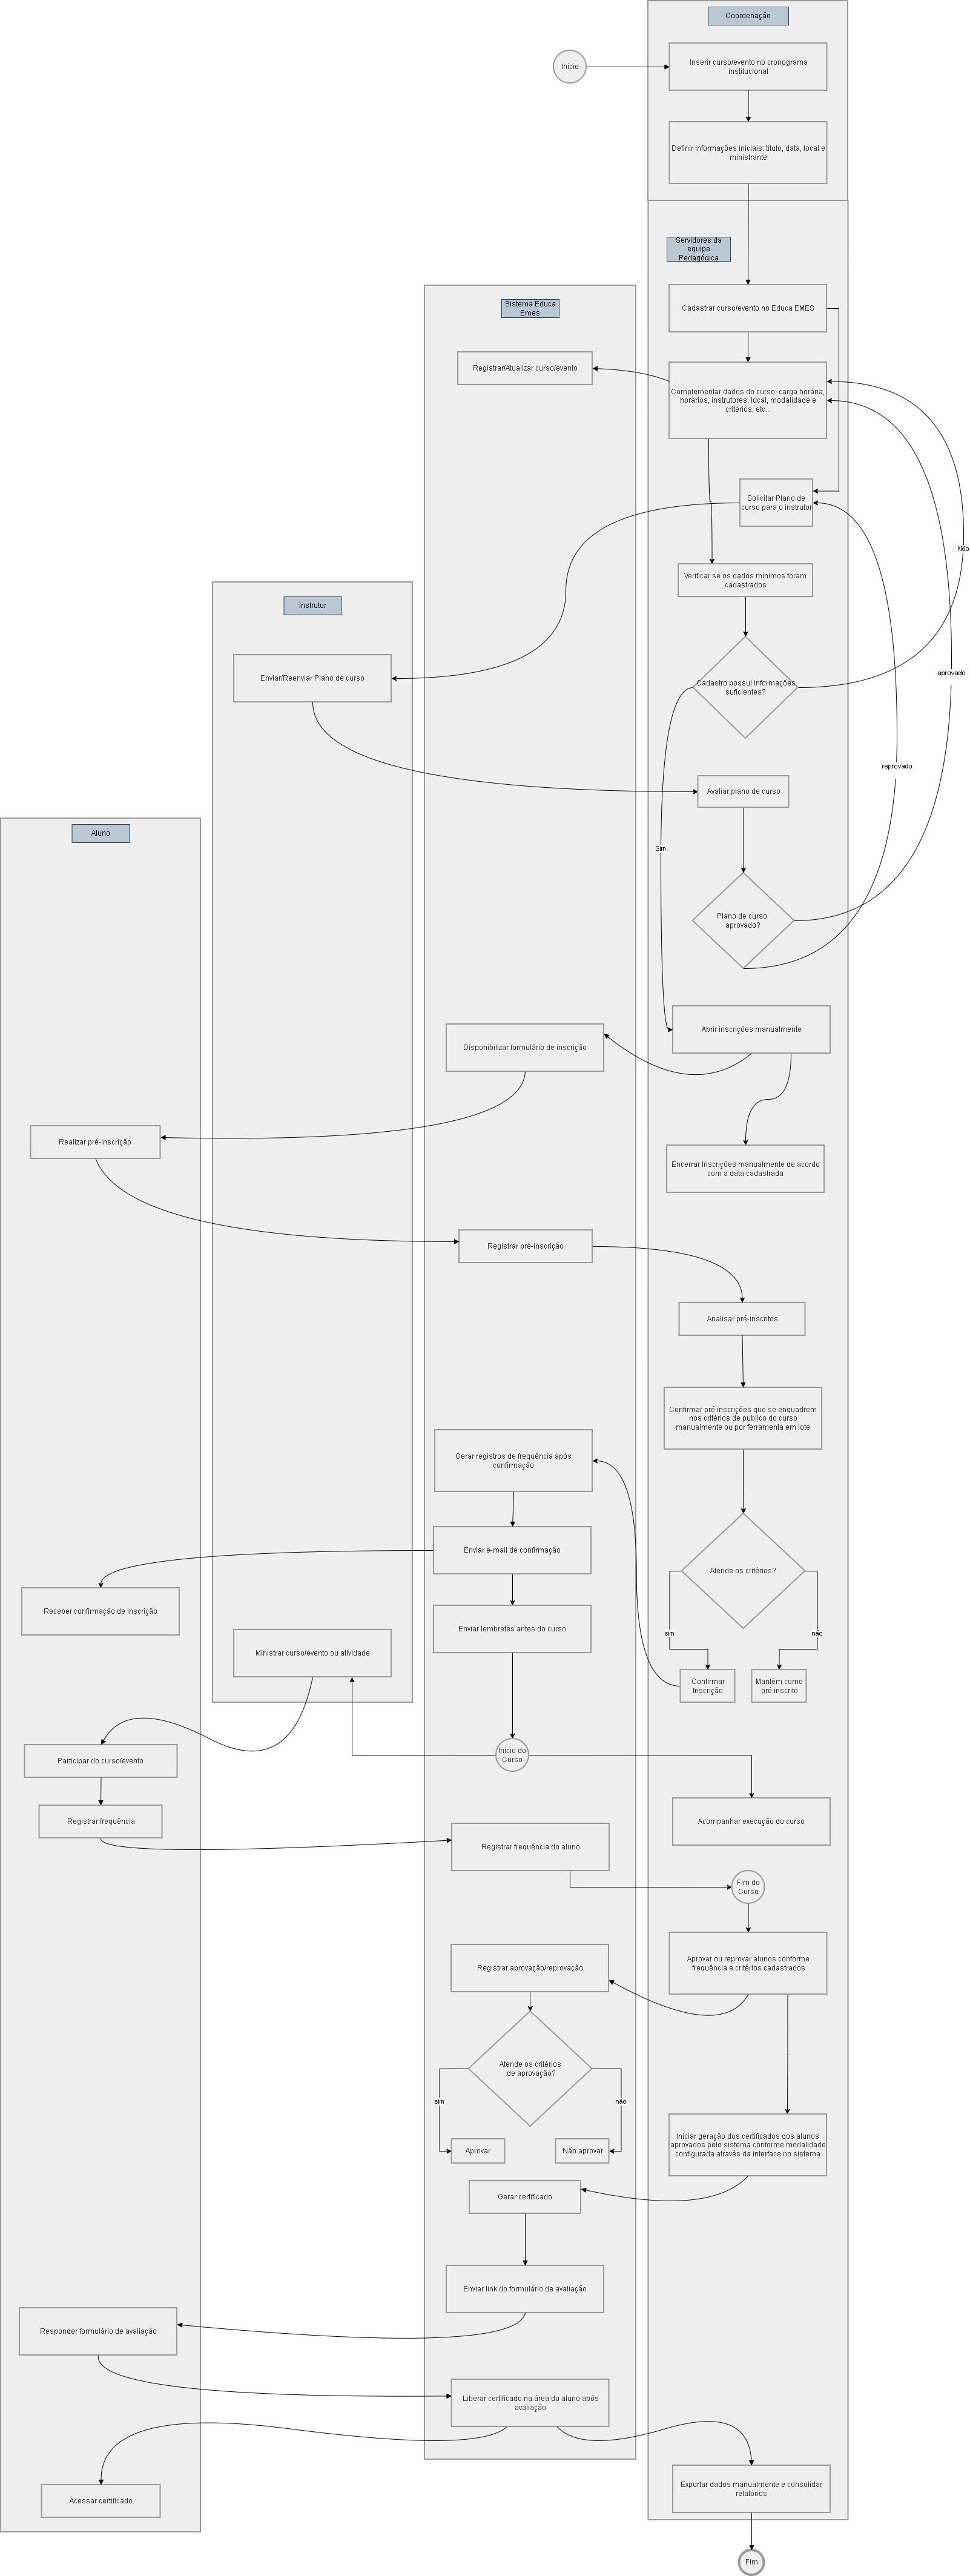
\includegraphics[scale=0.13]{imagens/bpmn-as-is.png}
  }
\end{figure}

O diagrama evidencia que o fluxo se inicia na coordenação, com a
inserção do curso ou evento no cronograma institucional, e avança para a
equipe pedagógica, responsável por complementar o cadastro no sistema,
avaliar informações adicionais, solicitar plano de curso ao instrutor e
acompanhar as etapas de inscrição, execução, aprovação, certificação e
consolidação de relatórios. Em paralelo, o sistema Educa EMES executa
atividades de apoio, como registro de curso, verificação de dados
mínimos, disponibilização de formulário de inscrição, geração de
registros de frequência, envio de e-mails e liberação de certificados.

Um aspecto relevante observado no modelo está na presença de gateways de
decisão concentrados principalmente na raia dos servidores da equipe
pedagógica, como nos pontos de aprovação do plano de curso e de análise
dos critérios para confirmação das pré-inscrições. Esses pontos indicam
dependência de avaliação humana em etapas centrais do processo,
caracterizando gargalos operacionais, especialmente quando há volume
elevado de cursos, necessidade de interpretação contextual ou ausência de
padronização dos critérios adotados. Além disso, a sequência associada à
abertura e ao encerramento manual das inscrições reforça a existência de
etapas sensíveis a esquecimento, atraso ou configuração inadequada.

Também se observa que, embora o sistema execute automaticamente algumas
ações após determinadas confirmações, como geração de registros de
frequência, envio de lembretes e disponibilização posterior de
certificados, o encadeamento geral do fluxo ainda depende de decisões
manuais em pontos estratégicos. Isso confirma que o problema investigado
não está na ausência de suporte computacional, mas na coexistência entre
automação parcial e intervenções humanas recorrentes em momentos críticos
do fluxo pedagógico.

\subsection{Síntese das etapas, gargalos e soluções propostas}
\label{sec:metod:etapas:sintese-gargalos}

Com base na análise do fluxo pedagógico atual, nos pontos de intervenção
manual identificados e nos gargalos observados, elaborou-se uma síntese
das principais etapas do processo, dos problemas recorrentes associados
a cada uma delas e das soluções propostas para seu tratamento no âmbito
da automação. Essa consolidação permite visualizar, de forma integrada,
como o diagnóstico do processo atual fundamenta a modelagem da solução
proposta.

\begin{table}[H]
\centering
\caption{Síntese entre etapas do fluxo pedagógico, gargalos e soluções propostas}
\label{tab:etapas-gargalos-solucoes}
\begin{tabular}{p{3.2cm} p{5.2cm} p{5.2cm}}
\hline
\textbf{Etapa do fluxo} & \textbf{Gargalo observado} & \textbf{Solução proposta} \\
\hline
Cadastro e planejamento do curso & Omissão de campos essenciais, conflitos de agenda e inconsistências de parametrização do curso. & Validações automáticas de integridade do cadastro, verificação de campos mínimos e alertas para pendências antes da execução. \\
\hline
Gestão de inscrições & Esquecimento na abertura ou encerramento das inscrições e configuração incorreta de datas. & Regras automáticas para abertura e encerramento conforme parâmetros configurados, com alertas e acompanhamento de status. \\
\hline
Confirmação de inscrições & Dependência de análise manual de perfis em cursos com públicos-alvo específicos. & Aplicação de critérios configuráveis de elegibilidade e apoio à confirmação automática ou semiautomática das inscrições. \\
\hline
Aprovação de participantes & Inconsistência de critérios de aprovação, especialmente em cursos com múltiplas atividades. & Padronização das regras de aprovação e processamento baseado em frequência e critérios previamente definidos. \\
\hline
Certificação & Divergências entre a modalidade cadastrada e a certificação efetivamente executada. & Geração orientada por regras de certificação vinculadas à configuração do curso e ao resultado da etapa de aprovação. \\
\hline
Relatórios e acompanhamento & Extração manual de dados para atendimento de demandas operacionais e gerenciais. & Consolidação automatizada de informações e geração de relatórios dinâmicos para acompanhamento do fluxo pedagógico. \\
\hline
\end{tabular}
\end{table}

\section{Análise do Sistema Atual}
\label{sec:metod:analise_sis}

A análise do sistema atual teve como objetivo compreender a estrutura
técnica do Educa EMES, identificando os principais componentes
tecnológicos, a organização da aplicação e o modelo de persistência
utilizado para sustentar o fluxo pedagógico. Essa etapa foi necessária
para contextualizar a proposta de automação dentro de uma solução já
existente, em funcionamento e integrada com diferentes rotinas
acadêmicas e administrativas da EMES.

\subsection{Arquitetura tecnológica da aplicação}
\label{sec:metod:analise_sis:arquitetura}

O Educa EMES é uma aplicação web desenvolvida em PHP \cite{PHP2024},
utilizando o framework Laravel como base arquitetural
\cite{Laravel2024}. A escolha por Laravel permite a organização da
aplicação segundo o padrão Model-View-Controller (MVC),
separando responsabilidades entre regras de negócio, persistência de
dados, controle de requisições e camada de apresentação. Além disso, o
sistema utiliza recursos do ecossistema Laravel, como Eloquent ORM para
mapeamento objeto-relacional, migrations e models para representação
das entidades do domínio, além de mecanismos de autenticação,
autorização, notificações, filas e comandos de console
\cite{Sommerville2011,CodingStyle2019,LaravelDocs2024,LaravelQueues2024,LaravelCommands2024}.

Na camada de interface administrativa, o sistema utiliza o Filament,
framework construído sobre Laravel, Livewire e Blade, empregado para
acelerar a construção de painéis administrativos, formulários, tabelas,
filtros e ações operacionais
\cite{Filament2024,FilamentAdminPanel2024,Livewire2024,Blade2024}. Essa
escolha é relevante para o contexto
da EMES porque grande parte das rotinas pedagógicas e administrativas
depende de interfaces internas de cadastro, acompanhamento,
validação e execução de procedimentos pelos servidores. Dessa forma, o
Filament atua como camada de operação do sistema, enquanto Laravel
concentra a estrutura da aplicação e as regras de negócio.

Sob o ponto de vista metodológico, essa arquitetura é relevante porque a
proposta de automação não se desenvolve como artefato isolado, mas como
evolução de uma aplicação já consolidada. Isso significa que qualquer
solução proposta precisa respeitar a organização existente da camada de
domínio, os padrões de implementação adotados e os mecanismos já
utilizados pelo sistema para processamento interno
\cite{Sommerville2011,Pressman2014}.

\subsection{Modelo de persistência e banco de dados}
\label{sec:metod:analise_sis:banco}

O sistema utiliza banco de dados relacional, com persistência
estruturada em MySQL/MariaDB \cite{MySQL2024}. O uso de um Sistema Gerenciador de Banco
de Dados relacional é adequado ao domínio analisado, uma vez que o
fluxo pedagógico depende de entidades fortemente relacionadas, como
cursos, atividades, inscrições, alunos, instrutores, frequências,
certificados, agendas, públicos-alvo, comunicações e avaliações. A
integridade dessas relações é essencial para garantir consistência
entre as etapas do processo acadêmico, especialmente nos pontos em que
uma ação posterior depende de registros anteriores, como a geração de
frequência a partir de uma inscrição confirmada ou a emissão de
certificados a partir da aprovação do aluno \cite{MySQL2024}.

A análise da estrutura de dados do Educa EMES foi realizada a partir do
esquema relacional do banco de dados e dos models da aplicação,
considerando o recorte diretamente relacionado ao fluxo pedagógico e
administrativo. Esse recorte incluiu as entidades responsáveis por
representar cursos, atividades, inscrições, participantes,
instrutores, frequências, certificados, agendas, públicos-alvo,
comunicações, arquivos, avaliações e tabelas auxiliares de
classificação.

Embora o banco de dados do sistema possua outras tabelas voltadas a
módulos administrativos, documentais, financeiros ou estruturas legadas,
tais elementos não foram considerados nesta etapa quando não
apresentavam relação direta com o ciclo pedagógico analisado. Essa
delimitação foi necessária para evitar que a análise estrutural se
transformasse em uma descrição completa de todo o banco de dados, o que
não contribuiria diretamente para os objetivos deste trabalho. Assim, o
foco foi direcionado às entidades que participam da criação, execução,
acompanhamento e encerramento de cursos e eventos educacionais.

\subsection{Entidades centrais do fluxo pedagógico}
\label{sec:metod:analise_sis:entidades}

O diagrama conceitual sintetizando as entidades principais do recorte
analisado foi deslocado para o
Apêndice~\ref{apend:diagramas-analise-sistema}, onde pode ser consultado
com melhor legibilidade.

A estrutura analisada demonstra que a tabela \texttt{esc\_cursos} ocupa
posição central no modelo de dados. Essa tabela armazena os principais
dados de planejamento e execução dos cursos, incluindo informações como
título, período de realização, carga horária, número de vagas, datas de
inscrição, modalidade, tipo de evento, local, critérios de aprovação,
liberação de inscrição, liberação de frequência e indicação de
certificação.

No modelo atual, a entidade de curso também é utilizada para representar
atividades vinculadas a um curso principal. Essa diferenciação ocorre
por meio do campo \texttt{curso\_id}: registros sem valor nesse campo
representam cursos ou eventos principais, enquanto registros com
\texttt{curso\_id} preenchido representam atividades associadas a outro
curso. Essa estratégia é reforçada nos models da aplicação, nos quais o
model \texttt{Cursos} aplica escopo para registros sem
\texttt{curso\_id}, enquanto o model \texttt{CursoAtividades} utiliza a
mesma tabela física, porém filtrando registros que possuem
\texttt{curso\_id} preenchido.

A partir da entidade central de cursos, o fluxo pedagógico se ramifica
para diferentes grupos de informações. O primeiro grupo corresponde aos
vínculos de participação, representados principalmente pela tabela
\texttt{esc\_cursoalunos}. Essa tabela relaciona usuários a cursos ou
atividades, armazenando dados como situação da inscrição, data de
inscrição, aprovação e observações. Ela é fundamental para representar
a entrada do participante no fluxo acadêmico, servindo como base para
etapas posteriores, como geração de frequência, aprovação e
certificação.

O segundo grupo corresponde ao controle de frequência, representado pela
tabela \texttt{esc\_cursofrequencias}. Essa estrutura associa curso,
aluno, agenda e situação de frequência. Dessa forma, a presença do
participante não é tratada como um dado isolado, mas como um registro
vinculado ao curso ou atividade e, quando aplicável, ao horário
correspondente na agenda.

O terceiro grupo é formado pelas entidades de certificação, tendo como
principal tabela \texttt{esc\_cursocertificados}. Essa estrutura vincula
uma pessoa a um curso ou atividade certificável, armazenando
informações como modelo de certificado, carga horária, arquivo gerado,
disponibilidade e validação. No fluxo pedagógico, essa entidade
representa a etapa final do ciclo acadêmico, pois depende de
informações anteriores relacionadas à inscrição, frequência e
aprovação.

O quarto grupo envolve as entidades de planejamento e apoio
administrativo. Nesse conjunto estão tabelas como \texttt{adm\_agenda},
\texttt{esc\_instrutores}, \texttt{esc\_cursopublico},
\texttt{esc\_recursos}, \texttt{esc\_cursoarquivos} e
\texttt{esc\_comunicacaocurso}. Essas estruturas complementam a entidade
de curso com informações necessárias para sua execução, como horários,
responsáveis, público-alvo, recursos necessários, arquivos de
divulgação e comunicações associadas.

\begin{table}[H]
\centering
\caption{Agrupamento das principais entidades analisadas}
\label{tab:agrupamento-entidades-fluxo}
\begin{tabular}{p{4cm} p{5cm} p{5cm}}
\hline
\textbf{Grupo} & \textbf{Principais tabelas} & \textbf{Papel no fluxo} \\
\hline
Núcleo pedagógico & \texttt{esc\_cursos} & Representa cursos, eventos e atividades educacionais. \\
\hline
Participação & \texttt{esc\_cursoalunos}, \texttt{users}, \texttt{user\_perfil} & Representa
alunos, inscrições, perfis e vínculos com cursos. \\
\hline
Execução e frequência & \texttt{adm\_agenda}, \texttt{esc\_cursofrequencias} & Controla horários,
agendas e presença dos participantes. \\
\hline
Certificação & \texttt{esc\_cursocertificados}, \texttt{esc\_certificadomodelos} & Registra
certificados emitidos, modelos utilizados e disponibilidade. \\
\hline
Apoio pedagógico-administrativo & \texttt{esc\_instrutores}, \texttt{esc\_cursopublico},
\texttt{esc\_recursos}, \texttt{esc\_cursoarquivos} & Complementa o planejamento e a execução dos cursos. \\
\hline
Classificação e parametrização & \texttt{cad\_tabelaapoio}, \texttt{settings} & Armazena
classificações, códigos e parâmetros utilizados pelo sistema. \\
\hline
Comunicação e avaliação & \texttt{esc\_comunicacao}, \texttt{esc\_comunicacaocurso}, \texttt{esc\_formavaliacao},
\texttt{esc\_formsubmissions} & Apoia comunicações institucionais e avaliação dos cursos. \\
\hline
\end{tabular}
\end{table}

\subsection{Relacionamentos e dependências entre entidades do fluxo pedagógico}
\label{sec:metod:analise_sis:relacionamentos}


Do ponto de vista do fluxo pedagógico, a estrutura de dados pode ser
compreendida como uma cadeia de dependências entre entidades. O curso ou
atividade é inicialmente cadastrado e parametrizado; em seguida, são
definidos seus públicos, instrutores, recursos, arquivos e agenda;
posteriormente, os participantes são vinculados por meio das
inscrições; durante a execução, são registrados os dados de frequência;
ao final, ocorre a aprovação dos participantes e a geração dos
certificados. Essa sequência evidencia que a automação proposta não
atua sobre uma entidade isolada, mas sobre um conjunto de registros
interdependentes.

\begin{figure}[H]
\centering
\caption{Representação do fluxo pedagógico}
\label{fig:fluxo-pedagogico}
  \fbox{
     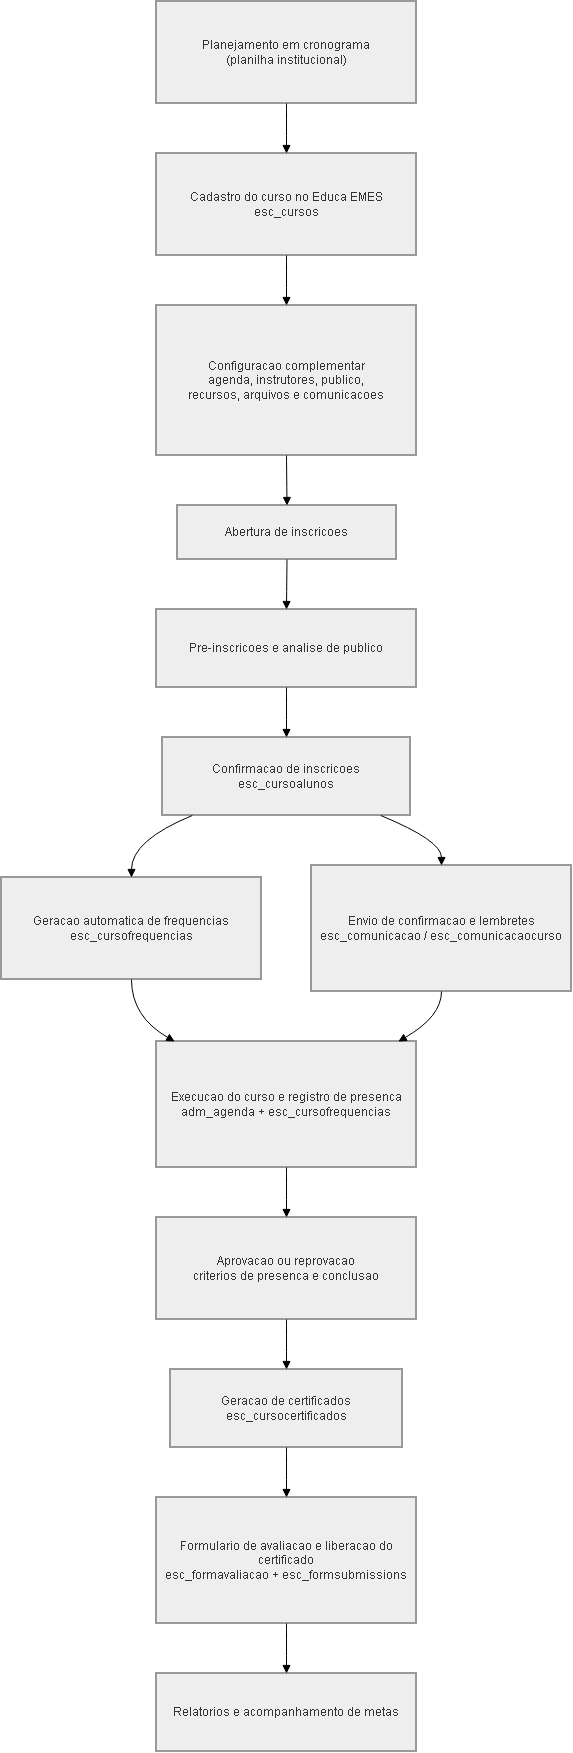
\includegraphics[scale=0.3]{imagens/fluxo-pedagogico.png}
  }
  % \legend{}
\end{figure}

O fluxo conceitual dos dados no ciclo pedagógico também foi organizado
no Apêndice~\ref{apend:diagramas-analise-sistema}, juntamente com o
modelo conceitual, a fim de concentrar os artefatos visuais de apoio à
análise estrutural do sistema em um único ponto de consulta.

\begin{table}[H]
\centering
\caption{Relação entre etapas do fluxo pedagógico e estruturas de dados}
\label{tab:fluxo-entidades-dados}
\begin{tabular}{p{4cm} p{5cm} p{5cm}}
\hline
\textbf{Etapa do fluxo} & \textbf{Entidades envolvidas} & \textbf{Dados necessários} \\
\hline
Planejamento do curso & \texttt{esc\_cursos}, \texttt{adm\_agenda}, \texttt{esc\_instrutores}
& Datas, horários, carga horária, local, instrutores e critérios. \\
\hline
Configuração do público & \texttt{esc\_cursopublico}, \texttt{user\_perfil},
\texttt{cad\_tabelaapoio} & Tipos de público, perfil dos usuários e classificações. \\
\hline
Inscrição & \texttt{esc\_cursoalunos}, \texttt{users} & Participante, curso,
situação da inscrição e data de inscrição. \\
\hline
Controle de frequência & \texttt{esc\_cursofrequencias}, \texttt{adm\_agenda}
& Participante, agenda, situação de frequência e observações. \\
\hline
Aprovação & \texttt{esc\_cursoalunos}, \texttt{esc\_cursofrequencias} &
Frequência, critérios de aprovação e status do participante. \\
\hline
Certificação & \texttt{esc\_cursocertificados}, \texttt{esc\_certificadomodelos}
& Pessoa certificada, carga horária, modelo, arquivo e disponibilidade. \\
\hline
Avaliação e encerramento & \texttt{esc\_formavaliacao}, \texttt{esc\_formsubmissions}
& Formulário, respostas, participante e curso avaliado. \\
\hline
\end{tabular}
\end{table}

A estrutura observada evidencia que o modelo de dados já possui
elementos suficientes para sustentar a automação gradual do fluxo
pedagógico. A existência de registros específicos para inscrições,
frequências, certificados, agendas, públicos e comunicações permite que
as etapas do processo sejam verificadas e atualizadas de forma
sistemática. Além disso, os campos de automação presentes na tabela de
cursos permitem registrar configurações, estados e diagnósticos do
processamento automatizado, evitando que a solução precise ser
construída como um mecanismo externo desconectado da base atual.

\subsection{Limitações estruturais observadas}
\label{sec:metod:analise_sis:limitacoes}

Apesar de a estrutura analisada fornecer base consistente para a
automação proposta, algumas limitações estruturais foram identificadas.
A primeira delas está na reutilização da tabela \texttt{esc\_cursos}
para representar simultaneamente cursos principais e atividades
vinculadas. Embora essa estratégia favoreça reaproveitamento de
estrutura, ela também introduz ambiguidade semântica, pois elementos com
papéis distintos no domínio passam a compartilhar a mesma representação
física \cite{Sommerville2011,Pressman2014}.

Outra limitação relevante está na centralização de múltiplas
classificações na tabela genérica \texttt{cad\_tabelaapoio}. Essa
abordagem oferece flexibilidade e reduz a proliferação de tabelas de
domínio, mas torna mais dependente da aplicação a interpretação correta
de grupos, códigos e significados utilizados em filtros, validações e
regras operacionais \cite{MySQL2024}.

Também se observou que os relacionamentos polimórficos, especialmente no
caso da agenda, ampliam a flexibilidade do modelo, porém reduzem a
capacidade de o próprio banco garantir integridade referencial de forma
explícita. Isso desloca parte importante da confiabilidade da relação
para a camada de aplicação, exigindo maior rigor na implementação e na
manutenção das regras de negócio \cite{LaravelDocs2024,Sommerville2011}.

Por fim, a própria natureza encadeada do fluxo pedagógico faz com que
inconsistências em etapas iniciais, como cadastro incompleto, agenda
incompatível ou parametrização inadequada do público e dos critérios de
aprovação, repercutam nas etapas posteriores de frequência,
certificação, comunicação e avaliação. Em razão disso, conclui-se que a
automação do fluxo pedagógico depende não apenas da existência das
entidades e relacionamentos, mas também da qualidade estrutural e da
coerência semântica com que esses elementos são configurados no sistema.

\section{Levantamento de requisitos}
\label{sec:metod:requisitos}

O levantamento de requisitos da proposta foi conduzido a partir da
análise do fluxo pedagógico atual, dos gargalos identificados e da
estrutura existente do sistema Educa EMES. Diferentemente de uma
especificação hipotética, os requisitos foram derivados de um sistema
real em produção e de rotinas institucionais observadas no contexto da
EMES. Essa abordagem permitiu definir funcionalidades aderentes ao
funcionamento efetivo da aplicação e aos pontos de intervenção manual
identificados nas etapas anteriores.

Nesta etapa, foram considerados os atores envolvidos no fluxo
pedagógico, os casos de uso associados à automação, os requisitos
funcionais necessários para ampliar o nível de automação e os requisitos
não funcionais relacionados à rastreabilidade, extensibilidade,
processamento assíncrono e separação de responsabilidades. Os diagramas
de apoio foram organizados com foco no comportamento esperado da
solução, enquanto os detalhes internos da arquitetura são tratados
posteriormente na seção de modelagem da solução proposta.

\begin{figure}[H]
\centering
\caption{Mapa de derivação do levantamento de requisitos}
\label{fig:mapa-requisitos}
  \fbox{
     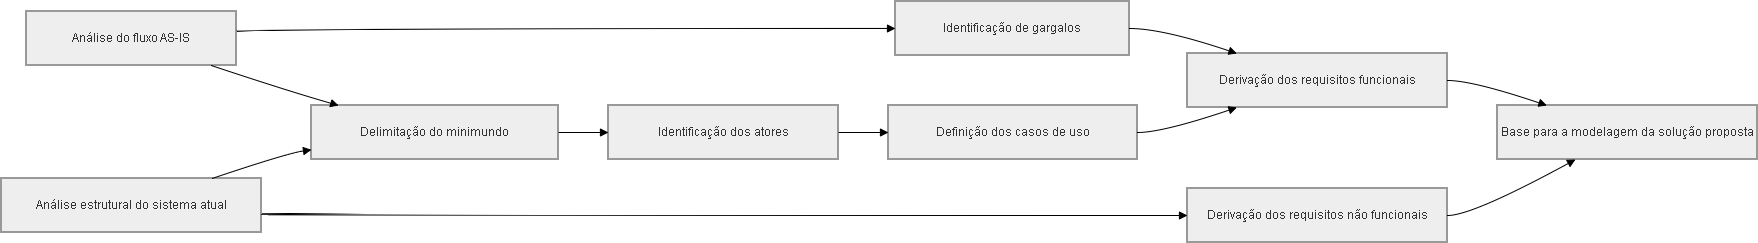
\includegraphics[scale=0.25]{imagens/mapa-requisitos.png}
  }
\end{figure}

\subsection{Delimitação do minimundo}
\label{sec:metod:requisitos:minimundo}

O minimundo considerado neste trabalho corresponde ao contexto de
gestão pedagógica da EMES, no qual o sistema é responsável por apoiar o
cadastro e a oferta de cursos, o controle de inscrições, o registro de
frequência, a certificação, a agenda acadêmica, a definição de
públicos-alvo, a comunicação institucional e a automação de etapas do
fluxo pedagógico.

Nesse domínio, cada curso pode possuir atividades vinculadas,
participantes, frequências, certificados, instrutores, recursos e
configurações automatizadas. O sistema também contempla regras
relacionadas a períodos de inscrição, critérios de aprovação, geração de
certificados, relatórios e disparo de notificações. Assim, o
levantamento de requisitos não trata de todo o Educa EMES, mas do
recorte diretamente relacionado ao fluxo pedagógico passível de
automação.

\subsection{Atores envolvidos}
\label{sec:metod:requisitos:atores}

Com base na análise do fluxo pedagógico, da estrutura funcional do
sistema e das rotinas institucionais observadas, foram identificados os
atores apresentados na
Tabela~\ref{tab:atores-levantamento-requisitos}.

\begin{table}[H]
\centering
\caption{Atores considerados no levantamento de requisitos}

\label{tab:atores-levantamento-requisitos}
\begin{tabular}{p{4cm} p{10cm}}
\hline

\textbf{Ator} & \textbf{Responsabilidade principal} \\
\hline
Equipe pedagógica & Cadastrar cursos, configurar parâmetros da automação, reutilizar configurações e acompanhar o andamento do fluxo automatizado. \\
\hline
\textbf{Responsáveis da equipe pedagógica} & Acompanhar o fluxo geral, receber notificações sobre pendências e erros, intervir manualmente e consultar o status da automação. \\
\hline
Aluno / participante & Realizar inscrição, participar do curso, registrar frequência e acessar certificado. \\
\hline
Sistema de automação pedagógica & Executar análise periódica, classificar o estado do curso, identificar etapas elegíveis, processar ações automatizadas e registrar notificações e status do fluxo. \\
\hline
\end{tabular}
\end{table}

\subsection{Casos de uso da automação}
\label{sec:metod:requisitos:casos-uso}

Os casos de uso da automação descrevem as funcionalidades esperadas da
solução sob a perspectiva dos atores externos e do comportamento
observável do sistema. Nesta etapa, o objetivo não é detalhar a
arquitetura interna da automação, mas explicitar a fronteira funcional do
problema e as capacidades necessárias para sustentar o fluxo pedagógico
automatizado.

\begin{figure}[H]
\centering
\caption{Casos de uso da automação pedagógica}
\label{fig:casos-uso-levantamento-requisitos}
  \fbox{
     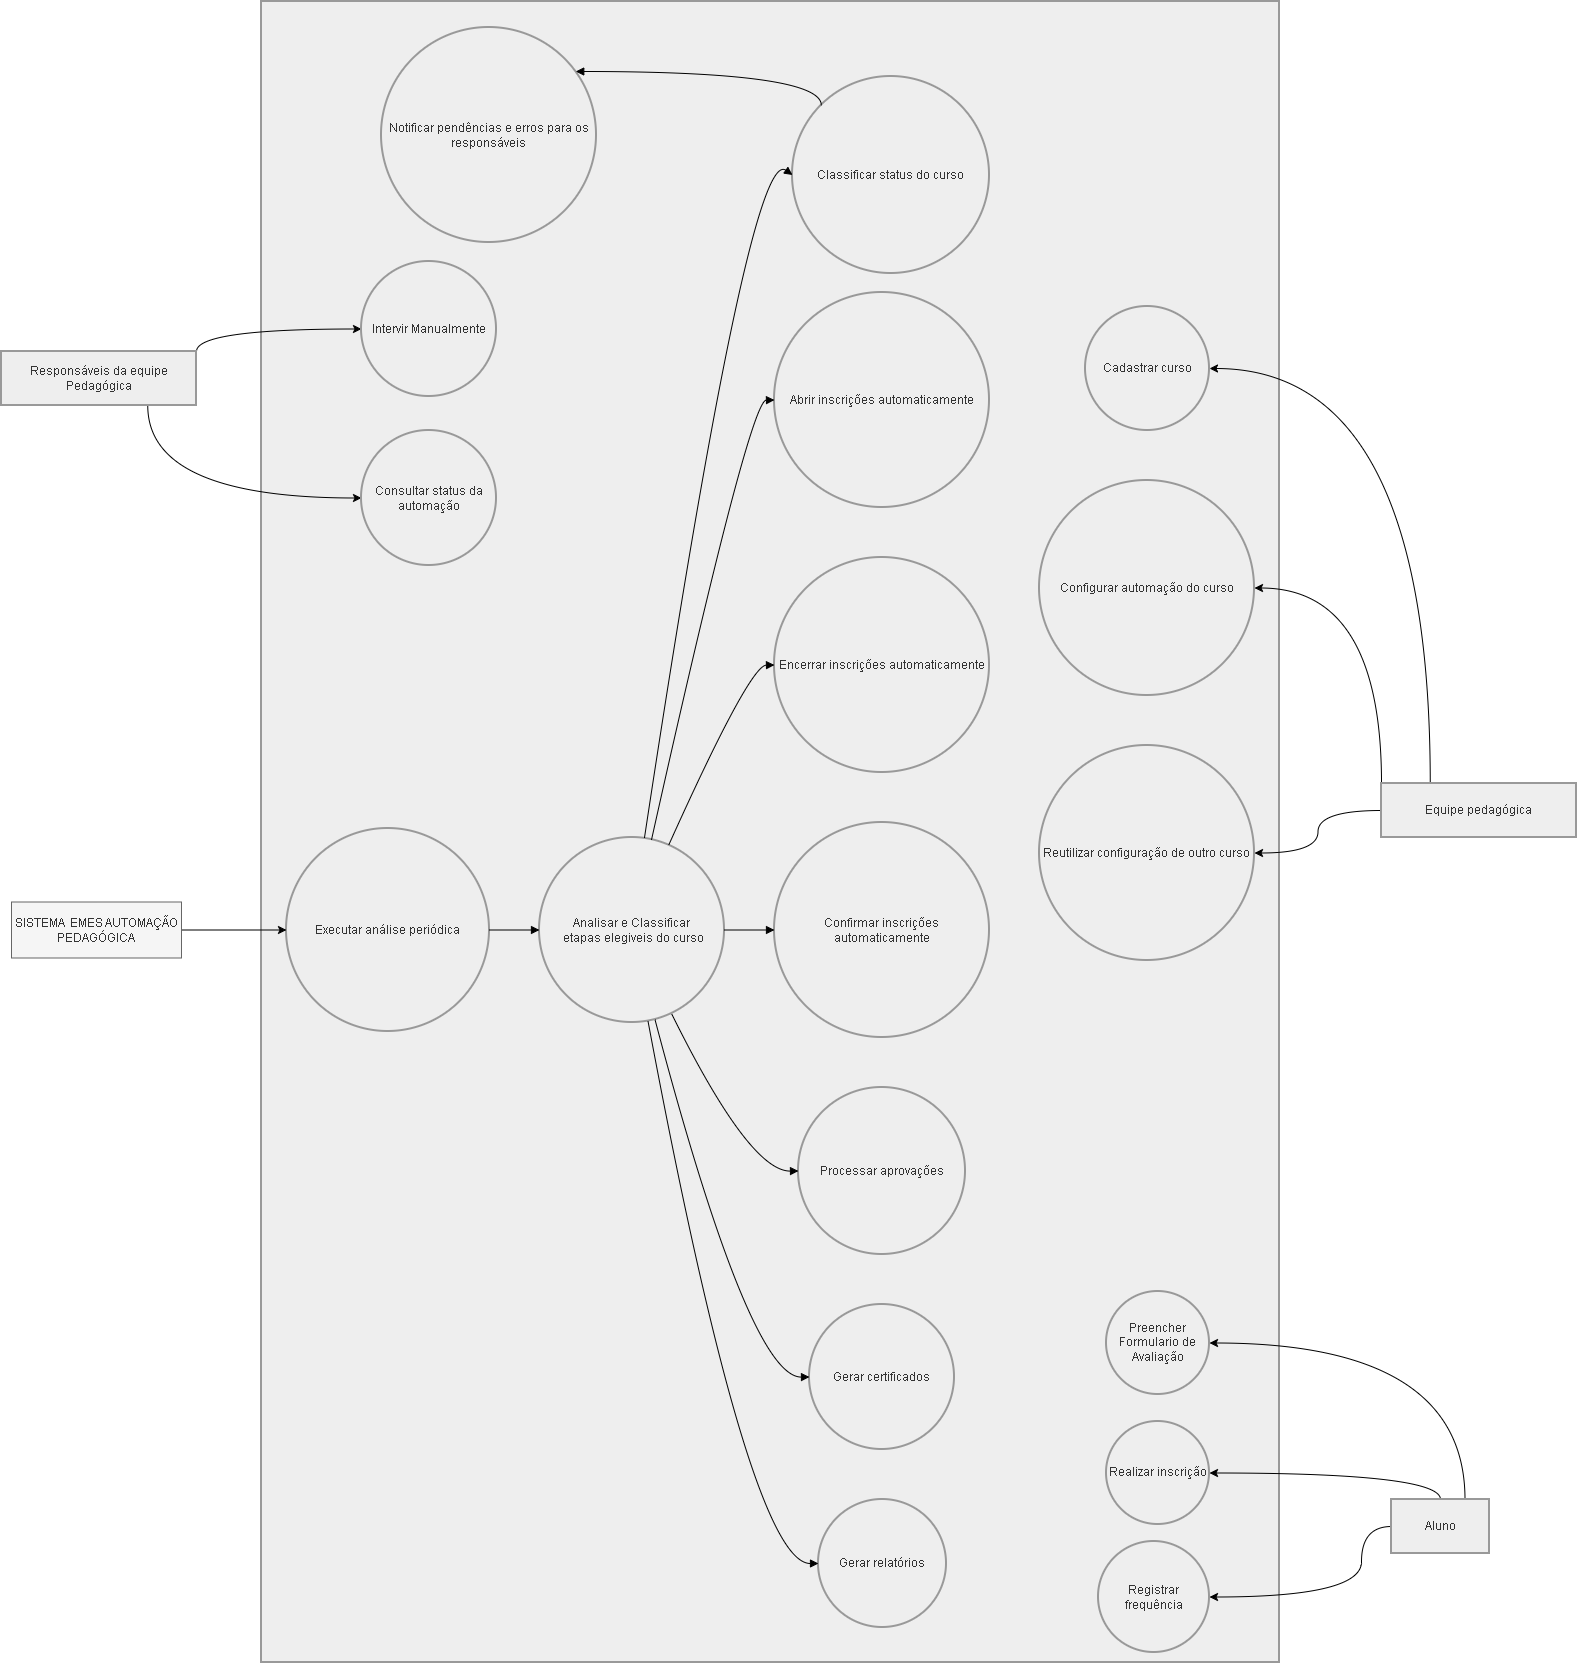
\includegraphics[scale=0.3]{imagens/caso-de-uso.png}
  }
\end{figure}

O diagrama evidencia que a equipe pedagógica atua no cadastro do curso,
na configuração da automação e na reutilização de configurações entre
cursos, enquanto os responsáveis da equipe pedagógica concentram as
ações de acompanhamento, consulta de status, notificação e intervenção
manual em situações de pendência. O sistema de automação pedagógica, por
sua vez, executa a análise periódica dos cursos, classifica o estado do
fluxo e apoia a abertura e o encerramento de inscrições, a confirmação
de participantes, o processamento de aprovações, a geração de
certificados e de relatórios, além da notificação de pendências e erros
aos responsáveis. O aluno permanece relacionado às interações esperadas
no fluxo, como realização de inscrição, registro de frequência e
preenchimento do formulário de avaliação.

\subsection{Requisitos funcionais}
\label{sec:metod:requisitos:funcionais}

Os requisitos funcionais foram derivados das capacidades observadas no
sistema e das operações necessárias para sustentar a automação do fluxo
pedagógico. A Tabela~\ref{tab:requisitos-funcionais-levantamento}
consolida os principais requisitos identificados, alinhados aos casos de
uso e às necessidades observadas no processo atual.

\begin{table}[H]
\centering
\caption{Requisitos funcionais identificados}
\label{tab:requisitos-funcionais-levantamento}
\begin{tabular}{p{2cm} p{11cm}}
\hline
\textbf{Código} & \textbf{Requisito funcional} \\
\hline
RF01 & O sistema deve permitir habilitar ou desabilitar a automação de um curso. \\
\hline
RF02 & O sistema deve permitir configurar regras automáticas relacionadas à inscrição, confirmação, aprovação, certificação e relatórios. \\
\hline
RF03 & O sistema deve analisar periodicamente cursos com automação habilitada. \\
\hline
RF04 & O sistema deve identificar etapas elegíveis para execução automática. \\
\hline
RF05 & O sistema deve registrar ações pendentes quando uma etapa não puder ser executada automaticamente. \\
\hline
RF06 & O sistema deve permitir intervenção manual em etapas bloqueadas ou pendentes. \\
\hline
RF07 & O sistema deve abrir inscrições automaticamente conforme parâmetros configurados. \\
\hline
RF08 & O sistema deve encerrar inscrições automaticamente conforme parâmetros configurados. \\
\hline
RF09 & O sistema deve confirmar inscrições com base em critérios previamente definidos. \\
\hline
RF10 & O sistema deve processar aprovação com base nos critérios de frequência e configuração do curso. \\
\hline
RF11 & O sistema deve gerar certificados conforme modalidade e critérios definidos no curso. \\
\hline
RF12 & O sistema deve gerar ou apoiar a geração de relatórios do fluxo pedagógico. \\
\hline
RF13 & O sistema deve notificar responsáveis sobre pendências, bloqueios e ações necessárias. \\
\hline
RF14 & O sistema deve manter histórico e status das etapas automatizadas. \\
\hline
RF15 & O sistema deve permitir configurar pontos de controle ou interrupção manual no fluxo. \\
\hline
\end{tabular}
\end{table}

\subsection{Requisitos não funcionais}
\label{sec:metod:requisitos:nao-funcionais}

Além das funcionalidades esperadas, a análise também evidenciou
propriedades estruturais e operacionais necessárias para que a solução
proposta seja sustentável, extensível e observável em ambiente real. Os
requisitos não funcionais identificados são apresentados na
Tabela~\ref{tab:requisitos-nao-funcionais-levantamento}, dialogando com
princípios de extensibilidade arquitetural, separação de
responsabilidades e processamento assíncrono discutidos na literatura
\cite{GammaEtAl1994,ServiceLayerPattern2024,LaravelQueues2024,LaravelScheduler2024}.
Esses requisitos fornecem base para a modelagem da solução proposta na
seção seguinte.

\begin{table}[H]
\centering
\caption{Requisitos não funcionais identificados}
\label{tab:requisitos-nao-funcionais-levantamento}
\begin{tabular}{p{2cm} p{12cm}}
\hline
\textbf{Código} & \textbf{Requisito não funcional} \\
\hline
RNF01 & O sistema deve possuir arquitetura extensível, baseada em estratégias de processamento. \\
\hline
RNF02 & O sistema deve registrar logs de execução, eventos relevantes e falhas ocorridas durante a automação. \\
\hline
RNF03 & O sistema deve suportar processamento assíncrono e agendado para execução periódica das análises. \\
\hline
RNF04 & O sistema deve manter rastreabilidade das etapas automatizadas e de seus respectivos estados. \\
\hline
RNF05 & O sistema deve permitir a expansão de novos fluxos automatizados sem necessidade de reestruturação ampla do núcleo da solução. \\
\hline
RNF06 & O sistema deve centralizar estruturas padronizadas de análise para reduzir inconsistências entre etapas. \\
\hline
RNF07 & O sistema deve separar responsabilidades de configuração, análise e execução das ações automatizadas. \\
\hline
RNF08 & O sistema deve preservar a possibilidade de intervenção manual sem comprometer a continuidade do fluxo automatizado. \\
\hline
RNF09 & O sistema deve manter consistência entre dados de inscrição, frequência, aprovação e certificação. \\
\hline
\end{tabular}
\end{table}

\subsection{Síntese dos fluxos analisados}
\label{sec:metod:requisitos:fluxos}

Os artefatos elaborados para esta etapa foram organizados de modo a
explicitar, sob diferentes perspectivas, como os requisitos da solução
foram derivados do fluxo pedagógico analisado e quais comportamentos são
esperados da automação proposta.

\begin{figure}[H]
\centering
\caption{Fluxo geral da automação no levantamento de requisitos}
\label{fig:fluxo-geral-automacao-requisitos}
  \fbox{
     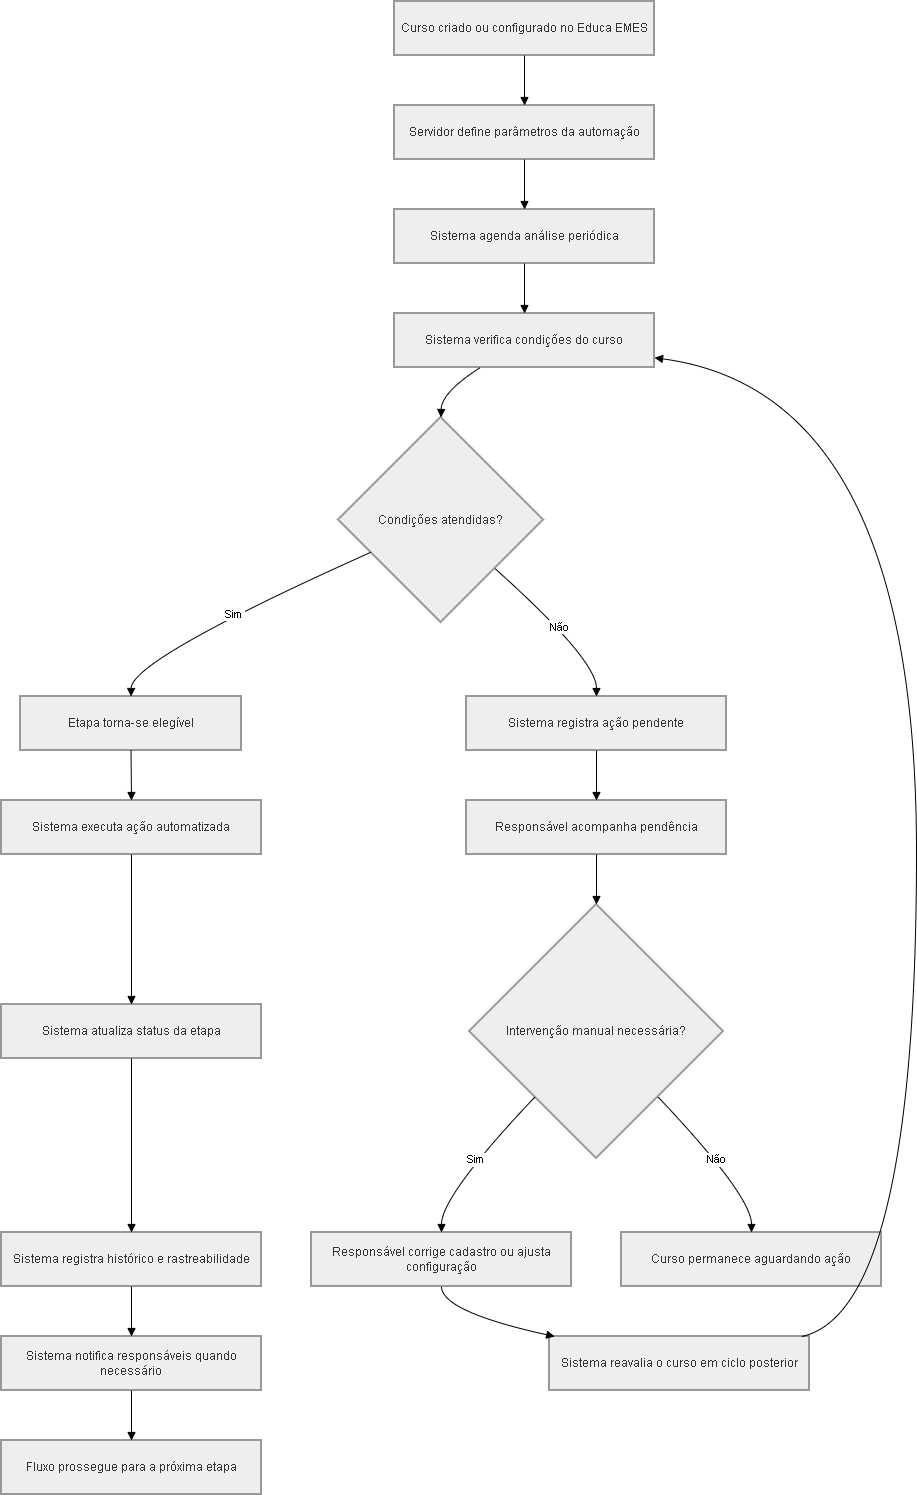
\includegraphics[scale=0.42]{imagens/fluxo-automacao.png}
  }
\end{figure}

\begin{figure}[H]
\centering
\caption{Sequência abstrata do comportamento esperado da automação}
\label{fig:sequencia-requisitos}
  \fbox{
     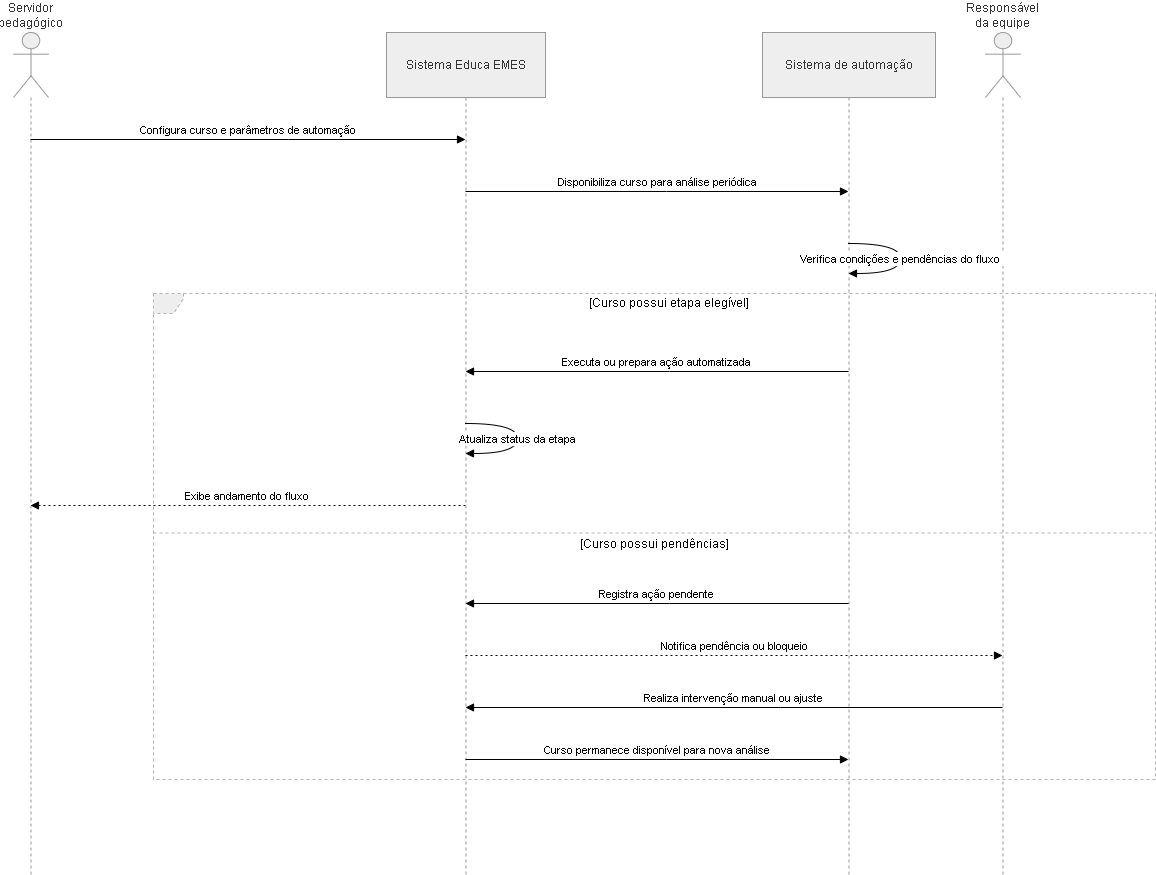
\includegraphics[scale=0.32]{imagens/diagrama-sequencia-requisitos.png}
  }
\end{figure}

O diagrama de casos de uso apresenta os atores externos e as
funcionalidades esperadas da solução. O fluxo geral da automação
representa o comportamento macro do processo automatizado, desde a
configuração do curso e a análise periódica das condições até a execução
da ação automatizada ou o registro de pendências. Já a sequência
abstrata representa a interação esperada entre servidor pedagógico,
sistema Educa EMES, sistema de automação e responsável da equipe, sem
antecipar os componentes internos da arquitetura.

Em conjunto, esses artefatos confirmam que o problema investigado não se
limita à execução isolada de tarefas, mas envolve a coordenação de um
fluxo contínuo de análise, decisão, intervenção e atualização de status
sobre entidades pedagógicas interdependentes. O mapa de derivação, os
casos de uso, o fluxo geral e a sequência abstrata mostram que os
requisitos levantados funcionam como ponte entre a análise do processo
atual e a modelagem da solução proposta, sustentando a evolução da
arquitetura apresentada na seção seguinte \cite{Pressman2014}.

\section{Modelagem da solução proposta}
\label{sec:metod:modelagem}

A modelagem da solução proposta foi elaborada com o objetivo de
estruturar um núcleo de automação capaz de analisar, classificar e
apoiar a execução das etapas do fluxo pedagógico do Educa EMES.
Diferentemente de uma automação pontual, limitada à execução isolada de
tarefas, a proposta organiza o fluxo em etapas configuráveis,
associadas a estados, critérios de elegibilidade, pendências e
possibilidades de intervenção manual.

A entidade curso foi adotada como unidade central da automação, uma vez
que concentra os principais dados relacionados ao planejamento,
execução, certificação e acompanhamento das ações pedagógicas. A partir
das informações vinculadas ao curso, o sistema pode analisar
inscrições, frequências, certificados, agenda, público-alvo e
parâmetros específicos de configuração, articulando a modelagem da
solução com a estrutura previamente identificada no sistema atual.

\subsection{Definição da stack e justificativa tecnológica}
\label{sec:metod:modelagem:stack}

A modelagem da solução parte da mesma base tecnológica adotada no
Educa EMES, uma vez que a automação proposta não constitui um sistema
paralelo, mas uma evolução incorporada à plataforma já existente. Essa
decisão considera dois fatores centrais: a familiaridade prática no
desenvolvimento com as ferramentas adotadas e a aderência à stack
nativa do sistema em que a automação será implementada.

\begin{table}[H]
\centering
\caption{Stack tecnológica considerada na modelagem da solução}
\label{tab:stack-modelagem-automacao}
\begin{tabular}{p{3cm} p{10cm}}
\hline
\textbf{Tecnologia} & \textbf{Papel na solução} \\
\hline
PHP & Linguagem principal da aplicação e base de implementação das regras da automação \cite{PHP2024}. \\
\hline
Laravel & Framework principal, responsável pela organização da aplicação, de serviços, comandos, filas, modelos e regras de domínio \cite{Laravel2024,LaravelCommands2024,LaravelQueues2024}. \\
\hline
Livewire & Suporte a componentes reativos utilizados nas interações administrativas da aplicação \cite{Livewire2024}. \\
\hline
Filament & Camada administrativa adotada no sistema para formulários, painéis, tabelas e operações internas de configuração e acompanhamento \cite{Filament2024,FilamentAdminPanel2024}. \\
\hline
MySQL/MariaDB & Sistema gerenciador de banco de dados relacional utilizado para persistência das entidades pedagógicas e dos estados da automação \cite{MySQL2024}. \\
\hline
\end{tabular}
\end{table}

Do ponto de vista arquitetural, a automação foi modelada sobre a
organização já presente no sistema, especialmente na separação entre
camada de domínio, serviços e persistência, no uso de comandos e
processamento agendado para orquestração e na centralidade da entidade
curso como agregadora do fluxo. Essa escolha reduz atrito de integração,
preserva consistência com a base existente e favorece a evolução
incremental da solução dentro do próprio Educa EMES.

\subsection{Visão geral da automação proposta}
\label{sec:metod:modelagem:visao-geral}

A solução proposta consiste na estruturação de um núcleo de automação
responsável por analisar periodicamente cursos com automação habilitada
e determinar quais etapas do fluxo pedagógico estão prontas para
execução, bloqueadas por pendências, aguardando intervenção manual ou
concluídas. Em vez de distribuir regras de negócio em rotinas isoladas,
a automação foi concebida como um fluxo recorrente de análise,
classificação, apoio à execução e atualização de status.

Essa visão responde diretamente aos requisitos levantados na seção
anterior, sobretudo aos requisitos relacionados à análise periódica de
cursos, identificação de etapas elegíveis, registro de pendências,
preservação da rastreabilidade e intervenção manual controlada. A
modelagem também considera que a automação não elimina a atuação humana,
mas a reorganiza em pontos de decisão, supervisão e tratamento de
exceções, o que a torna mais aderente ao contexto institucional
observado na EMES.

\subsection{Modelo de etapas automatizadas}
\label{sec:metod:modelagem:etapas}

A proposta organiza o fluxo em seis etapas principais de automação,
correspondentes aos pontos de maior recorrência operacional e maior
potencial de padronização identificados ao longo da análise do processo
atual.

\begin{table}[H]
\centering
\caption{Etapas automatizadas consideradas na modelagem da solução}
\label{tab:etapas-modelagem-automacao}
\begin{tabular}{p{4cm} p{9cm}}
\hline
\textbf{Etapa} & \textbf{Finalidade principal} \\
\hline
\texttt{abrir\_inscricao} & Verificar se o curso atingiu as condições necessárias para abertura automática do período de inscrição. \\
\hline
\texttt{encerrar\_inscricao} & Verificar se o período de inscrição deve ser encerrado conforme os parâmetros definidos para o curso. \\
\hline
\texttt{confirmar\_inscricao} & Avaliar critérios de elegibilidade e apoiar a confirmação de participantes previamente inscritos. \\
\hline
\texttt{processar\_aprovacoes} & Aplicar critérios de frequência e aprovação para consolidação do resultado acadêmico do participante. \\
\hline
\texttt{gerar\_certificados} & Verificar condições de certificação e apoiar a emissão de certificados conforme a modalidade configurada. \\
\hline
\texttt{gerar\_relatorios} & Consolidar informações do fluxo pedagógico para acompanhamento gerencial e apoio à tomada de decisão. \\
\hline
\end{tabular}
\end{table}

Cada uma dessas etapas compartilha uma estrutura comum de controle,
histórico, metadados e análise, ainda que possua regras próprias de
elegibilidade e de bloqueio. Essa padronização permite tratar as etapas
como unidades comparáveis dentro do mesmo fluxo, favorecendo
rastreabilidade, manutenção e expansão gradual do núcleo da automação.

\subsection{Estados e transições das etapas}
\label{sec:metod:modelagem:estados}

Para que a automação não se reduza a uma execução linear de tarefas, a
modelagem prevê estados explícitos para as etapas. Esses estados
descrevem não apenas se uma ação foi executada, mas também se ela está
habilitada, pronta para execução, concluída, bloqueada, em erro ou
dependente de intervenção humana.

\begin{table}[H]
\centering
\caption{Estados previstos para as etapas da automação}
\label{tab:estados-etapas-automacao}
\begin{tabular}{p{3.5cm} p{9.5cm}}
\hline
\textbf{Estado} & \textbf{Significado} \\
\hline
\texttt{pending} & A etapa ainda não está pronta para execução. \\
\hline
\texttt{ready} & A etapa está elegível para execução. \\
\hline
\texttt{running} & A etapa está em execução. \\
\hline
\texttt{completed} & A etapa foi concluída com sucesso. \\
\hline
\texttt{blocked} & A etapa possui impedimentos que bloqueiam sua execução. \\
\hline
\texttt{awaiting\_action} & A etapa depende de intervenção manual ou decisão humana. \\
\hline
\texttt{error} & A etapa falhou durante análise ou execução. \\
\hline
\texttt{skipped} & A etapa foi ignorada por configuração ou regra de negócio. \\
\hline
\end{tabular}
\end{table}

Esse modelo por estados permite representar transições como
\texttt{pending} para \texttt{ready}, \texttt{ready} para
\texttt{running}, \texttt{running} para \texttt{completed}, bem como
transições motivadas por bloqueios, erros ou interrupção manual. Com
isso, a automação deixa de ser interpretada apenas como disparo de
ações e passa a ser tratada como um processo controlado por estados,
mais coerente com os requisitos de rastreabilidade e governança do
fluxo.

\subsection{Arquitetura do núcleo de automação}
\label{sec:metod:modelagem:arquitetura}

Em termos arquiteturais, a solução foi organizada em componentes com
responsabilidades especializadas, articulados em torno do curso e de seu
estado de automação. O processamento periódico inicia-se a partir de um
comando orquestrador, responsável por localizar cursos com automação
habilitada e acionar o serviço de análise. Esse serviço, por sua vez,
interpreta a configuração do curso, reconcilia as etapas do fluxo,
consolida diagnósticos, registra pendências e identifica etapas
elegíveis para execução.

Essa organização busca separar responsabilidades de configuração,
análise, classificação e execução, em consonância com os requisitos não
funcionais definidos anteriormente. A solução também favorece a
extensibilidade, pois o comportamento específico de cada etapa não fica
acoplado ao fluxo inteiro, mas distribuído em componentes modulares
voltados à interpretação de regras particulares.

\subsection{Responsabilidades dos componentes}
\label{sec:metod:modelagem:componentes}

O núcleo da automação foi modelado com base em um conjunto de classes e
componentes especializados, cada um com papel definido na interpretação
e no suporte à execução do fluxo pedagógico automatizado.

\begin{table}[H]
\centering
\caption{Componentes centrais da modelagem da automação}
\label{tab:componentes-modelagem-automacao}
\begin{tabular}{p{4.5cm} p{8.5cm}}
\hline
\textbf{Componente} & \textbf{Responsabilidade principal} \\
\hline
\texttt{ProcessarCursos} & Atuar como ponto de entrada do processamento periódico, selecionando cursos com automação habilitada e iniciando a análise do fluxo. \\
\hline
\texttt{CursoAnalyzerService} & Interpretar o estado atual do curso, ler \texttt{auto\_config}, reconciliar \texttt{auto\_steps}, consolidar diagnósticos, pendências e etapas elegíveis. \\
\hline
\texttt{StepStrategyInterface} & Definir o contrato comum das estratégias utilizadas para análise das etapas automatizadas. \\
\hline
\texttt{StepStrategyFactory} & Mapear cada etapa para sua strategy correspondente e isolar o serviço de análise do conhecimento direto sobre classes concretas. \\
\hline
\texttt{CertificarStepStrategy} e demais strategies & Aplicar regras específicas de elegibilidade, bloqueio e atualização de estado para cada etapa do fluxo. \\
\hline
\texttt{AutoStructureBuilder} & Centralizar a criação de estruturas padronizadas de etapa, análise, diagnóstico e \textit{pending actions}. \\
\hline
\texttt{CursoClassifierService} & Definir o status global da automação do curso a partir do resultado consolidado da análise. \\
\hline
\texttt{AutoNotificationService} &   Apoiar a comunicação com responsáveis em situações de pendência, erro, intervenção manual ou eventos relevantes do fluxo. \\
\hline
Jobs de execução & Executar ações potencialmente mais pesadas ou assíncronas relacionadas às etapas elegíveis do fluxo. \\
\hline
\end{tabular}
\end{table}

Essa distribuição de responsabilidades foi orientada pelos padrões
Strategy, Factory, Builder, Service Layer e Command, que permitem
organizar regras de negócio em serviços especializados, reduzir
acoplamento e ampliar a capacidade de evolução da solução sem
reestruturação ampla do núcleo.

\subsection{Tratamento de pendências e intervenção manual}
\label{sec:metod:modelagem:pendencias}

Um aspecto central da modelagem está no tratamento de pendências
identificadas durante a análise da automação. Em vez de assumir que toda
etapa elegível deve ser executada automaticamente, a solução registra
\textit{pending actions} sempre que encontra condições que bloqueiam,
desaconselham ou exigem revisão humana antes da continuidade do fluxo.

Essas pendências funcionam como mecanismo de governança do processo,
pois tornam visíveis situações como datas ausentes, critérios de
aprovação não configurados, inconsistências de agenda, ausência de
modelo de certificado ou necessidade de validação por responsável.
Nesses cenários, a etapa pode assumir o estado
\texttt{awaiting\_action}, preservando a possibilidade de intervenção
manual sem romper a rastreabilidade do fluxo automatizado.

Essa decisão é coerente com o contexto da EMES, onde diferentes cursos
podem apresentar exceções institucionais, especificidades pedagógicas ou
dependências informacionais não resolvidas apenas por regras fixas. A
automação, portanto, não foi modelada para substituir integralmente a
atuação humana, mas para apoiar a coordenação do fluxo, sinalizar
anomalias e reduzir retrabalho administrativo.

\subsection{Persistência da configuração e do estado da automação}
\label{sec:metod:modelagem:persistencia}

Do ponto de vista da persistência, a solução foi modelada com base em
quatro elementos principais associados ao curso: \texttt{auto},
\texttt{auto\_config}, \texttt{auto\_steps} e \texttt{auto\_status}. O
campo \texttt{auto} indica se a automação está habilitada para o curso;
\texttt{auto\_config} armazena os parâmetros configuráveis da automação;
\texttt{auto\_steps} registra o estado individual de cada etapa; e
\texttt{auto\_status} sintetiza a situação global do fluxo automatizado.

Essa estratégia reforça a centralidade da entidade curso na modelagem da
solução e evita a criação de um mecanismo paralelo desconectado da base
existente. Ao manter configuração, diagnóstico e status vinculados ao
próprio curso, a solução preserva aderência ao modelo de dados do Educa
EMES e amplia a capacidade de acompanhamento, auditoria e evolução
gradual da automação.

\subsection{Representação BPMN do fluxo pedagógico proposto}
\label{sec:metod:modelagem:bpmn-to-be}

Como complemento à representação \textit{AS-IS} apresentada na
Figura~\ref{fig:bpmn-as-is}, foi elaborado um diagrama BPMN
\textit{TO-BE}, apresentado na Figura~\ref{fig:bpmn-to-be}, com o
objetivo de representar o comportamento esperado do fluxo pedagógico
após a incorporação do núcleo de automação. O diagrama mantém a
organização por raias, mas redistribui responsabilidades entre
coordenação, equipe pedagógica, sistema Educa EMES, instrutor e aluno, de
modo a evidenciar quais decisões permanecem sob responsabilidade humana
e quais passam a ser tratadas pelo sistema. Assim como na representação
do fluxo atual, o instrutor aparece como participante do processo
pedagógico, sem assumir papel funcional direto na automação modelada.

\begin{figure}[H]
\centering
\caption{Representação BPMN do fluxo pedagógico proposto (\textit{TO-BE})}
\label{fig:bpmn-to-be}
  \fbox{
     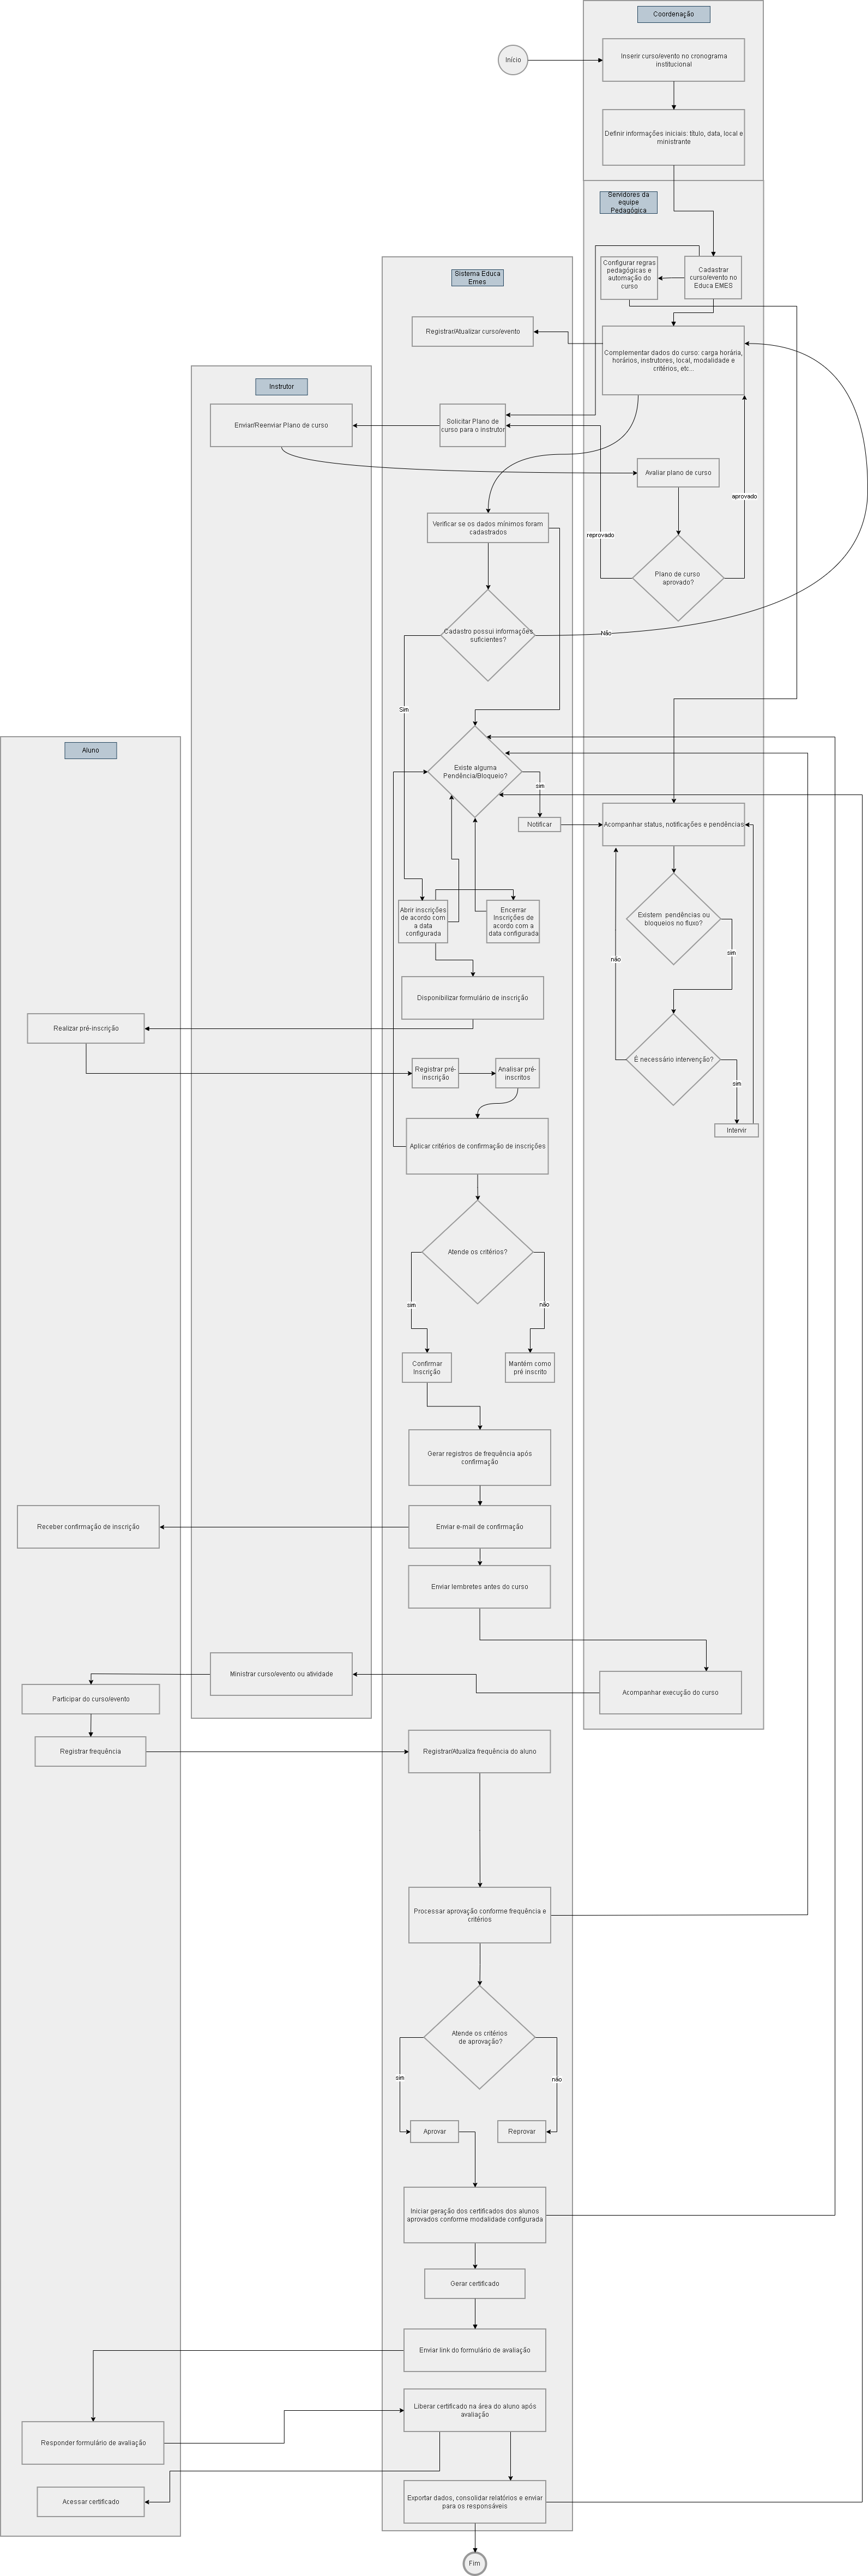
\includegraphics[width=0.95\textwidth,height=0.85\textheight,keepaspectratio]{imagens/bpmn-to-be.png}
  }
\end{figure}

A principal mudança em relação ao modelo \textit{AS-IS} está na
transferência de decisões operacionais recorrentes para a raia do sistema
Educa EMES. No fluxo atual, diversos gateways e atividades relativas à validação de
cadastro, abertura e encerramento de inscrições, confirmação de
participantes, aprovação, certificação e geração de relatórios dependem
de ação direta da equipe pedagógica. No fluxo proposto, essas verificações
passam a ser representadas como atividades sistemáticas de análise,
classificação e execução automatizada, orientadas pelas configurações do
curso e pelos estados das etapas.

Essa redistribuição não elimina a participação da equipe pedagógica. Ao
contrário, o modelo \textit{TO-BE} reposiciona os servidores em funções de
configuração, acompanhamento e intervenção. A equipe continua responsável
por cadastrar e complementar informações do curso, configurar regras
pedagógicas da automação, avaliar exceções e intervir quando o sistema
identificar pendências, bloqueios ou necessidade de decisão humana. Dessa
forma, os gateways deslocados para o sistema não indicam ausência de
governança, mas uma mudança no ponto de controle: o sistema passa a
detectar condições e encaminhar o fluxo, enquanto os responsáveis atuam
principalmente sobre exceções e validações que exigem julgamento
pedagógico.

Outro ponto relevante do diagrama é a presença explícita de mecanismos de
notificação e acompanhamento de status. Sempre que o sistema identifica
pendências ou bloqueios, o fluxo direciona a informação aos responsáveis,
preservando a possibilidade de intervenção manual antes da continuidade
da automação. Essa característica reforça a proposta de uma automação
assistida, na qual a execução automática das etapas é condicionada à
consistência dos dados e à ausência de impedimentos relevantes.

Sob essa perspectiva, o BPMN \textit{TO-BE} sintetiza a transição de um
processo dependente de decisões manuais recorrentes para um fluxo
orientado por regras configuráveis, estados de automação, pendências
registradas e intervenções controladas. Essa representação visual
consolida a modelagem apresentada nesta seção e explicita o resultado
esperado da solução: um fluxo pedagógico mais automatizado, rastreável e
orientado por exceções controladas.

% \section{Implementação da solução proposta}
% \label{sec:metod:implementacao}
